% Exact LaTeX recreation of the supplied Phase-1.pdf
% Compile with pdfLaTeX. Place member pictures in the same folder if required.

\documentclass[11pt,a4paper]{article}

\usepackage[a4paper,left=2.0cm,right=2.0cm,top=1.55cm,bottom=1.55cm]{geometry}
\usepackage[T1]{fontenc}
\usepackage{lmodern}
\usepackage{graphicx}
\usepackage{xcolor}
\usepackage{array}
\usepackage{tabularx}
\usepackage{ragged2e}
\usepackage{enumitem}
\usepackage{fancyhdr}
\usepackage{tikz}
\usetikzlibrary{positioning}
\usepackage{setspace}

% -------------------------------------------------
% COLOURS
% -------------------------------------------------
\definecolor{TitleBlue}{RGB}{61,103,154}

% -------------------------------------------------
% GENERAL SETTINGS
% -------------------------------------------------
\setlength{\parindent}{0pt}
\setlength{\parskip}{0pt}
\renewcommand{\arraystretch}{1.0}

% The supplied document uses a clean sans-serif heading style
% and italic serif-style explanatory text.
\newcommand{\blueheading}[1]{%
    {\sffamily\color{TitleBlue}\fontsize{15}{18}\selectfont #1}%
}

\newcommand{\bluebigheading}[1]{%
    {\sffamily\bfseries\color{TitleBlue}\fontsize{16}{19}\selectfont #1}%
}

\newcommand{\instruction}[1]{%
    {\itshape\fontsize{10.5}{12.5}\selectfont #1}%
}

\newsavebox{\answerboxcontent}
\newcommand{\answerbox}[2][3.0cm]{%
    % Measure the actual height of the answer at the box width.
    \sbox{\answerboxcontent}{%
        \begin{minipage}[t]{\dimexpr\textwidth-2\fboxsep-2\fboxrule\relax}
            \itshape #2
        \end{minipage}%
    }%
    \vspace{2pt}
    \noindent
    \fbox{%
        \begin{minipage}[t]{\dimexpr\textwidth-2\fboxsep-2\fboxrule\relax}
            \vspace{1mm}%
            \itshape #2
            \ifdim\ht\answerboxcontent<#1
                \vspace{\dimexpr#1-\ht\answerboxcontent\relax}%
            \fi
            \vspace{1mm}%
        \end{minipage}
    }
}

% -------------------------------------------------
% HEADER / FOOTER
% -------------------------------------------------
\pagestyle{fancy}
\fancyhf{}
\renewcommand{\headrulewidth}{0pt}
\renewcommand{\footrulewidth}{0pt}

\fancyhead[L]{%
    \sffamily\bfseries\itshape\fontsize{10.5}{12}\selectfont
    Data Structure And Programing In C++ DSCPP-III-2026-T037
}
\fancyhead[R]{%
    \sffamily\bfseries\fontsize{10.5}{12}\selectfont
    Bus Route Optimizer
}
\fancyfoot[R]{%
    \itshape\fontsize{10}{12}\selectfont
    Page \thepage
}
\setlength{\headheight}{14pt}
\setlength{\headsep}{23pt}
\setlength{\footskip}{24pt}

% -------------------------------------------------
% PAGE 1
% -------------------------------------------------
\begin{document}

\vspace*{4mm}

\bluebigheading{PROJECT AND TEAM INFORMATION}

\vspace{13mm}

\blueheading{Project Title}

\vspace{1mm}

\instruction{(Try to choose a catchy title. Max 20 words).}

\answerbox[1.0cm]{\textbf{Bus Route Optimizer}}

\vspace{13mm}

\blueheading{Student / Team Information}

\vspace{2mm}

% Team information table
% Compact 4-member layout so all members remain on Page 1.
\noindent
\begin{tabularx}{\textwidth}{|>{\RaggedRight\arraybackslash}p{0.69\textwidth}|>{\RaggedRight\arraybackslash}X|}
\hline
\begin{minipage}[t]{\linewidth}
\vspace{1.5mm}
\textit{Team Name:}\\[-1mm]
\textit{Team \#}
\vspace{1.5mm}
\end{minipage}
&
\begin{minipage}[t]{\linewidth}
\vspace{1.5mm}
\textit{Members}
\vspace{1.5mm}
\end{minipage}
\\
\hline
\begin{minipage}[t][3.25cm][t]{\linewidth}
\vspace{1.5mm}
\textbf{Team member 1 (Team Lead)}\\[-1mm]
\textit{(Last Name, name: student ID: email, picture):}
\vspace{2.0cm}
\end{minipage}
&
\begin{minipage}[t][3.25cm][t]{\linewidth}
\vspace{1.5mm}
\textit{Kant, Krishna -- 2510380211}\\
\textit{2510380211@geu.ac.in}

\vspace{2mm}
\IfFileExists{MEM1.png}{\includegraphics[width=3.0cm,height=1.5cm,keepaspectratio]{MEM1.png}}{\fbox{\rule{0pt}{1.5cm}\rule{3.0cm}{0pt}}}
\end{minipage}
\\
\hline
\begin{minipage}[t][3.25cm][t]{\linewidth}
\vspace{1.5mm}
\textbf{Team member 2}\\[-1mm]
\textit{(Last Name, name: student ID: email, picture):}
\vspace{2.0cm}
\end{minipage}
&
\begin{minipage}[t][3.25cm][t]{\linewidth}
\vspace{1.5mm}
\textit{Mishra, Agrima -- 2512510019}\\
\textit{2512510019@geu.ac.in}

\vspace{2mm}
\IfFileExists{MEM2.png}{\includegraphics[width=3.0cm,height=1.5cm,keepaspectratio]{MEM2.png}}{\fbox{\rule{0pt}{1.5cm}\rule{3.0cm}{0pt}}}
\end{minipage}
\\
\hline
\begin{minipage}[t][3.25cm][t]{\linewidth}
\vspace{1.5mm}
\textbf{Team member 3}\\[-1mm]
\textit{(Last Name, name: student ID: email, picture):}
\vspace{2.0cm}
\end{minipage}
&
\begin{minipage}[t][3.25cm][t]{\linewidth}
\vspace{1.5mm}
\textit{Singh, Aditi -- 2510012426}\\
\textit{2510012426@geu.ac.in}

\vspace{2mm}
\IfFileExists{MEM3.png}{\includegraphics[width=3.0cm,height=1.5cm,keepaspectratio]{MEM3.png}}{\fbox{\rule{0pt}{1.5cm}\rule{3.0cm}{0pt}}}
\end{minipage}
\\
\hline
\begin{minipage}[t][3.25cm][t]{\linewidth}
\vspace{1.5mm}
\textbf{Team member 4}\\[-1mm]
\textit{(Last Name, name: student ID: email, picture):}
\vspace{2.0cm}
\end{minipage}
&
\begin{minipage}[t][3.25cm][t]{\linewidth}
\vspace{1.5mm}
\textit{Gahlawat, Akhil -- 2510012465}\\
\textit{2510012465@geu.ac.in}

\vspace{2mm}
 \IfFileExists{MEM4.png}{\includegraphics[width=3.0cm,height=1.5cm,keepaspectratio]{MEM4.png}}{\fbox{\rule{0pt}{1.5cm}\rule{3.0cm}{0pt}}}
\end{minipage}
\\
\hline
\end{tabularx}

\newpage

% -------------------------------------------------
% PAGE 2
% -------------------------------------------------

\bluebigheading{PROPOSAL DESCRIPTION (10 pts)}

\vspace{12mm}

\blueheading{Motivation (1 pt)}

\vspace{1mm}

\instruction{(Describe the problem you want to solve and why it is important. Max 300 words).}

\answerbox[3.0cm]{%
In a city, buses operate through multiple routes and stops, making it difficult for passengers to determine the most suitable route between two locations. Finding the shortest or most efficient route manually can be time-consuming, especially when several bus stops and connections are involved. The Bus Route Optimizer aims to provide a simple system for managing bus routes and helping users find suitable routes between bus stops. The project will represent bus stops and their connections using a graph, where stops are vertices and roads are weighted edges. Algorithms such as Breadth First Search (BFS) and Dijkstra’s algorithm will be used to find routes with fewer stops and the shortest-distance route respectively. The system will also provide bus searching, ticket booking, cancellation, and waiting-list management. This project is important because it demonstrates how Data Structures and Algorithms can be applied to solve a practical transportation problem while using Object-Oriented Programming to organize the system efficiently.
}

\vspace{12mm}

\blueheading{State of the Art / Current solution (1 pt)}

\vspace{1mm}

\instruction{(Describe how the problem is solved today (if it is). Max 200 words).}

\answerbox[2.75cm]{%
Currently, passengers generally use navigation and public transportation applications to find routes between locations. These systems use large databases containing road networks, bus schedules, traffic information, and transportation data to provide route recommendations. However, such systems are complex and contain many features that are beyond the scope of a basic academic project. Our project provides a simplified implementation focused on the fundamental concepts of Data Structures and Algorithms. Bus stops will be represented as vertices of a graph, while connections between stops will be represented as weighted edges. BFS can be used to find a route with the minimum number of stops, while Dijkstra’s algorithm can find the shortest route based on distance. The system will also demonstrate basic bus and passenger management using Object-Oriented Programming.
}

\vspace{12mm}

\blueheading{Project Goals and Milestones (2 pts)}

\vspace{1mm}

\instruction{(Describe the project general goals. Include initial milestones as well any other milestones. Max 300 words).}

\answerbox[3.15cm]{%
The main goal of the Bus Route Optimizer is to develop a C++ based system that manages buses, bus stops, routes, and passengers while applying important Data Structures and Algorithms. The system will provide users with route-searching and shortest-path functionality.

\textbf{Initial milestones:}
\begin{enumerate}[leftmargin=*,nosep]
\item Analyze the problem and identify system requirements.
\item Design the classes for Bus, BusStop, Route, Passenger, and Graph.
\item Implement bus and bus-stop management.
\item Implement the graph using an adjacency list.
\item Implement BFS for finding routes with minimum stops.
\item Implement Dijkstra’s algorithm with a priority queue for shortest-distance routes.
\item Implement bus searching and route selection.
\item Implement ticket booking, cancellation, and waiting-list management using queues.
\item Integrate all modules through an Admin and User menu.
\item Test the complete system and prepare documentation and presentation.
\end{enumerate}
}

\vspace{12mm}

\blueheading{Project Approach (3 pts)}

\vspace{1mm}

\instruction{(Describe how you plan to articulate and design a solution. Including platforms and technologies that you will use. Max}

\instruction{300 words).}

\answerbox[3.05cm]{%
The project will be developed using C++ and will combine Object-Oriented Programming with Data Structures and Algorithms. Object-Oriented Programming will be used to represent major entities such as Bus, BusStop, Route, Passenger, and Graph through classes. Encapsulation will be used to protect class data and public member functions will provide controlled access.

The bus network will be represented using a weighted graph implemented through an adjacency list. Each bus stop will be treated as a vertex, while a connection between two stops will be an edge whose weight represents distance. BFS will be implemented using a queue to find routes requiring the minimum number of stops. Dijkstra’s algorithm, supported by a priority queue, will be used to calculate the shortest-distance route. Vectors will be used to store buses, stops, routes, and passengers, while a queue will be used for the passenger waiting list.

The system will provide separate Admin and User interfaces through a console-based application. The Admin will manage buses, stops, and routes, while users will search buses, find routes, and manage bookings. The project will initially be implemented in a single C++ source file and can later be divided into multiple .h and .cpp files for better organization.
}

\newpage

% -------------------------------------------------
% PAGE 3
% -------------------------------------------------

\blueheading{System Architecture (High Level Diagram)(2 pts)}

\vspace{1mm}

\instruction{(Provide an overview of the system, identifying its main components and interfaces in the form of a diagram using a tool}

\instruction{of your choice).}

\answerbox[4.0cm]{%
\centering
\begin{tikzpicture}[node distance=7mm and 11mm, >=stealth, every node/.style={font=\scriptsize\sffamily}, 
box/.style={draw, rounded corners, align=center, minimum height=7mm, text width=2.0cm},
algo/.style={draw, rounded corners, align=center, minimum height=7mm, text width=2.3cm}]
\node[box] (system) {Bus Route\\Optimizer};
\node[box, below left=of system] (admin) {Admin\\Interface};
\node[box, below right=of system] (user) {User\\Interface};
\node[box, below=of admin] (management) {Bus, Stop \&\\Route Management};
\node[box, below=of user] (services) {Bus Search \&\\Ticket Booking};
\node[box, below=of management] (graph) {Weighted Graph\\Adjacency List};
\node[algo, below left=of graph] (bfs) {BFS\\Minimum Stops};
\node[algo, below right=of graph] (dijkstra) {Dijkstra\\Shortest Distance};

\draw[->] (system) -- (admin);
\draw[->] (system) -- (user);
\draw[->] (admin) -- (management);
\draw[->] (user) -- (services);
\draw[->] (management) -- (graph);
\draw[->] (services) -- (graph);
\draw[->] (graph) -- (bfs);
\draw[->] (graph) -- (dijkstra);
\end{tikzpicture}

\vspace{2mm}

\raggedright
The system consists of Admin and User interfaces connected to the management, bus-search, booking, and graph modules. The graph module uses an adjacency list and supports BFS and Dijkstra’s algorithm for route optimization.
}

\vspace{12mm}

\blueheading{Project Outcome / Deliverables (1 pts)}

\vspace{1mm}

\instruction{(Describe what are the outcomes / deliverables of the project. Max 200 words).}

\answerbox[2.7cm]{%
The final outcome will be a functional console-based Bus Route Optimizer developed in C++. The system will allow administrators to add and manage buses, bus stops, and routes. Users will be able to search for buses and find routes between selected bus stops. The project will implement a graph using an adjacency list and provide two route-finding approaches: BFS for finding routes with the minimum number of stops and Dijkstra’s algorithm for finding the shortest route based on distance. A priority queue will be used in Dijkstra’s algorithm and a queue will be used for passenger waiting-list management. The system will also support passenger ticket booking, cancellation, seat management, and basic fare calculation. The major deliverables will include the C++ source code, system architecture, project documentation, test results, and a presentation demonstrating the working system and the DSA and OOP concepts used.
}

\vspace{12mm}

\blueheading{Assumptions}

\vspace{6mm}

\instruction{( Describe the assumptions ( if any ) you are making to solve the problem. Max 100 words )}

\answerbox[2.65cm]{%
\begin{enumerate}[leftmargin=*,nosep]
\item Bus stops and routes are predefined or entered by the administrator.
\item The distance between connected bus stops is known and fixed.
\item Each bus has a fixed seating capacity.
\item Buses operate on predefined routes.
\item All route distances are positive.
\item Real-time traffic, weather, and road conditions are not considered.
\item Users provide valid source and destination bus stops.
\item Ticket booking depends on seat availability.
\item Passengers are added to a waiting queue when the bus is full.
\item The system is an academic simulation and does not include real-time GPS tracking or online payment.
\end{enumerate}
}

\vspace{12mm}

\blueheading{References}

\vspace{1mm}

\instruction{(Provide a list of resources or references you utilised for the completion of this deliverable. You may provide links).}

\answerbox[2.65cm]{%
\begin{enumerate}[leftmargin=*,nosep]
\item Thomas H. Cormen, Charles E. Leiserson, Ronald L. Rivest, and Clifford Stein, \textit{Introduction to Algorithms}, MIT Press.
\item Bjarne Stroustrup, \textit{The C++ Programming Language}, Addison-Wesley.
\item C++ Reference --- documentation for C++ language and Standard Library.
\item Course lecture notes and materials on Data Structures and Object-Oriented Programming.
\item Graph algorithms and shortest-path algorithm study materials.
\end{enumerate}
}

\end{document}
